\documentclass[xcolor={dvipsnames}]{beamer}

\usetheme{Malmoe}
\usecolortheme{seagull}
\usepackage[]{natbib}
\usepackage{textpos}
\usepackage{amsmath, amssymb, bm}
\usepackage{multirow}
\usepackage{framed}
\usepackage{schemata}
\setbeamertemplate{navigation symbols}{}
\usepackage[english]{babel}
\usepackage{animate}
\usepackage{graphics}
\usepackage{fontawesome}


\definecolor{lightblue}{rgb}{0.145,0.6666,1} % Defines the color used for content box headers
\definecolor{Red}{rgb}{0.9,0.15,0}
\definecolor{Blue}{RGB}{55,126,184}
\definecolor{Green}{RGB}{77,175,74}
\definecolor{White}{RGB}{255,255,255}
\definecolor{Lightgray}{rgb}{0.86,0.86,0.86}

\setbeamertemplate{footline}
{
	\leavevmode%
	\hbox{%
		\begin{beamercolorbox}[wd=.50\paperwidth,ht=2.25ex,dp=1ex,center]{author in head/foot}%
			\usebeamerfont{author in head/foot}\insertshortauthor%% \beamer@ifempty{\insertshortinstitute}{}{(\insertshortinstitute)}
		\end{beamercolorbox}%
%		\hskip2pt%
		\begin{beamercolorbox}[wd=.50\paperwidth,ht=2.25ex,dp=1ex,center]{title in head/foot}%
			\usebeamerfont{title in head/foot}\insertshorttitle~~~~~~~~~~~~~~~~~~~~~~~~~~\insertframenumber
		\end{beamercolorbox}%
	}%
	\vskip0pt%
}
\makeatother

\title[Violencia y demograf\'ia]{
	\small{\textsl{}}\\$\,$\\$\,$}

\subtitle{\large{\textsc{La epidemia de violencia en M\'exico y su impacto en la salud de la poblaci\'on:\\
 Una perspectiva demogr\'afica’}}\\$\,$\\}


\author[CIDE, 5 de Marzo]
{
	\vspace{-0.5cm}
	\texorpdfstring{
		\begin{columns}
			\column{.9\linewidth}
			\centering
			\normalsize{Jos\'{e} Manuel Aburto}\\
			$\,$\\
			
\includegraphics[scale=0.12]{Figures/logos.png}     
		\end{columns}
	}
	{Jos\'{e} Manuel Aburto}
}

\date[]{}

\beamertemplatenavigationsymbolsempty
\begin{document}


\begin{frame}[plain]
	\titlepage
\end{frame}
%%%%%%%%%%%%%%%%%%%%%%%%%%%%%%%%%%%%%%%%%%%%%%%%%%%%%%%%%%%%%%%%%%%%%%%%%
%%%%%%%%%%%%%%%%%%%%%%%%%%%%%%%%%%%%%%%%%%%%%%%%%%%%%%%%%%%%%%%%%%%%%%%%%
\section{Aumento de la violencia}

%%%%%%%%%%%%%%%%%%%%%%%%%%%%%%%%%%%%%%%%%%%%%%%%%%%%%%%%%%%%%%%%%%%%%%%%%
\begin{frame}
\Large{
		\begin{itemize}
		
		\item<1-> \textbf{La violencia} es un problema prioritario en Am\'erica Latina.
		
		\item<2-> Am\'erica Latina tiene la tasa \textbf{m\'as alta} de homicidios en el mundo (16.3 per 100,000).
		
        \item<3-> \textbf{Recrudecimiento} de homicidios en el siglo XXI.

        \item<4-> En M\'exico, las tasas se \textbf{duplicaron} entre 2007 y 2012 (9.3 $\longrightarrow$ 18.6).
		
		\end{itemize}
		
}

\end{frame}

\section{Impacto de la violencia en la salud}

\begin{frame}
\Large{
		\begin{itemize}
		    
		\item Esperanza de vida en hombres se \textbf{estanc\'o} en la d\'ecada de 2000-10 ($\backsim $72y)
		
				\end{itemize}
		
		\pause
				\begin{center}
		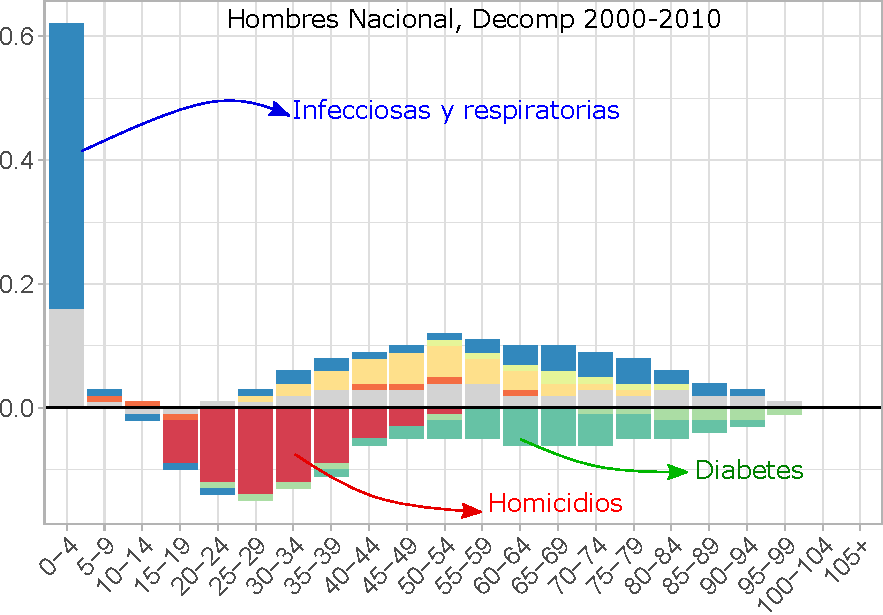
\includegraphics[scale=.55]{Figures/Fig_1}
				\end{center}
				

}
\end{frame}

\begin{frame}



\hbox{\hspace{-2em}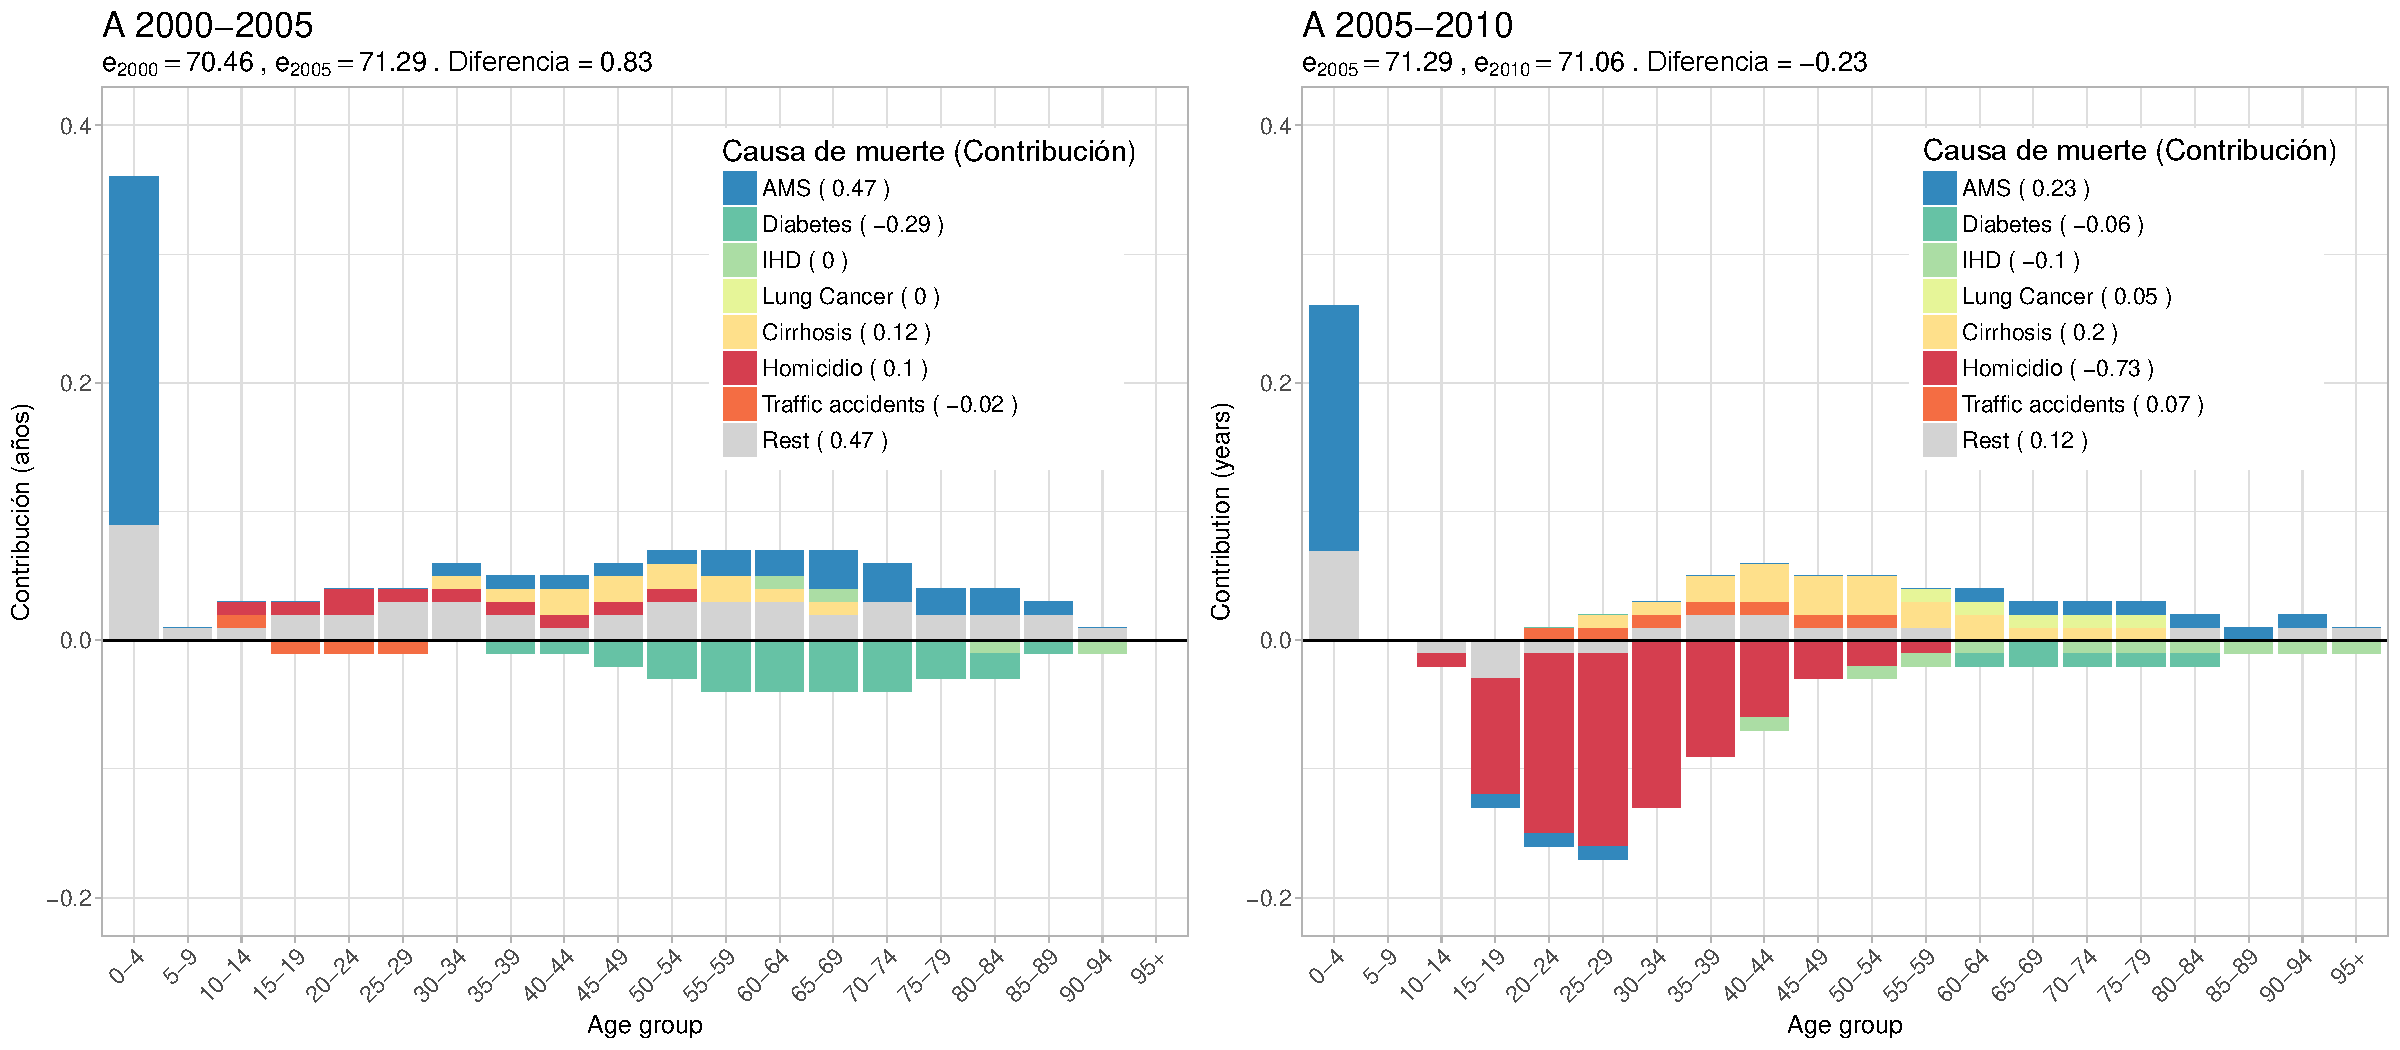
\includegraphics[scale=.3]{Figures/Fig2}}

				

\end{frame}



\begin{frame} \frametitle{Propagaci\'on de la violencia}
\begin{center}
		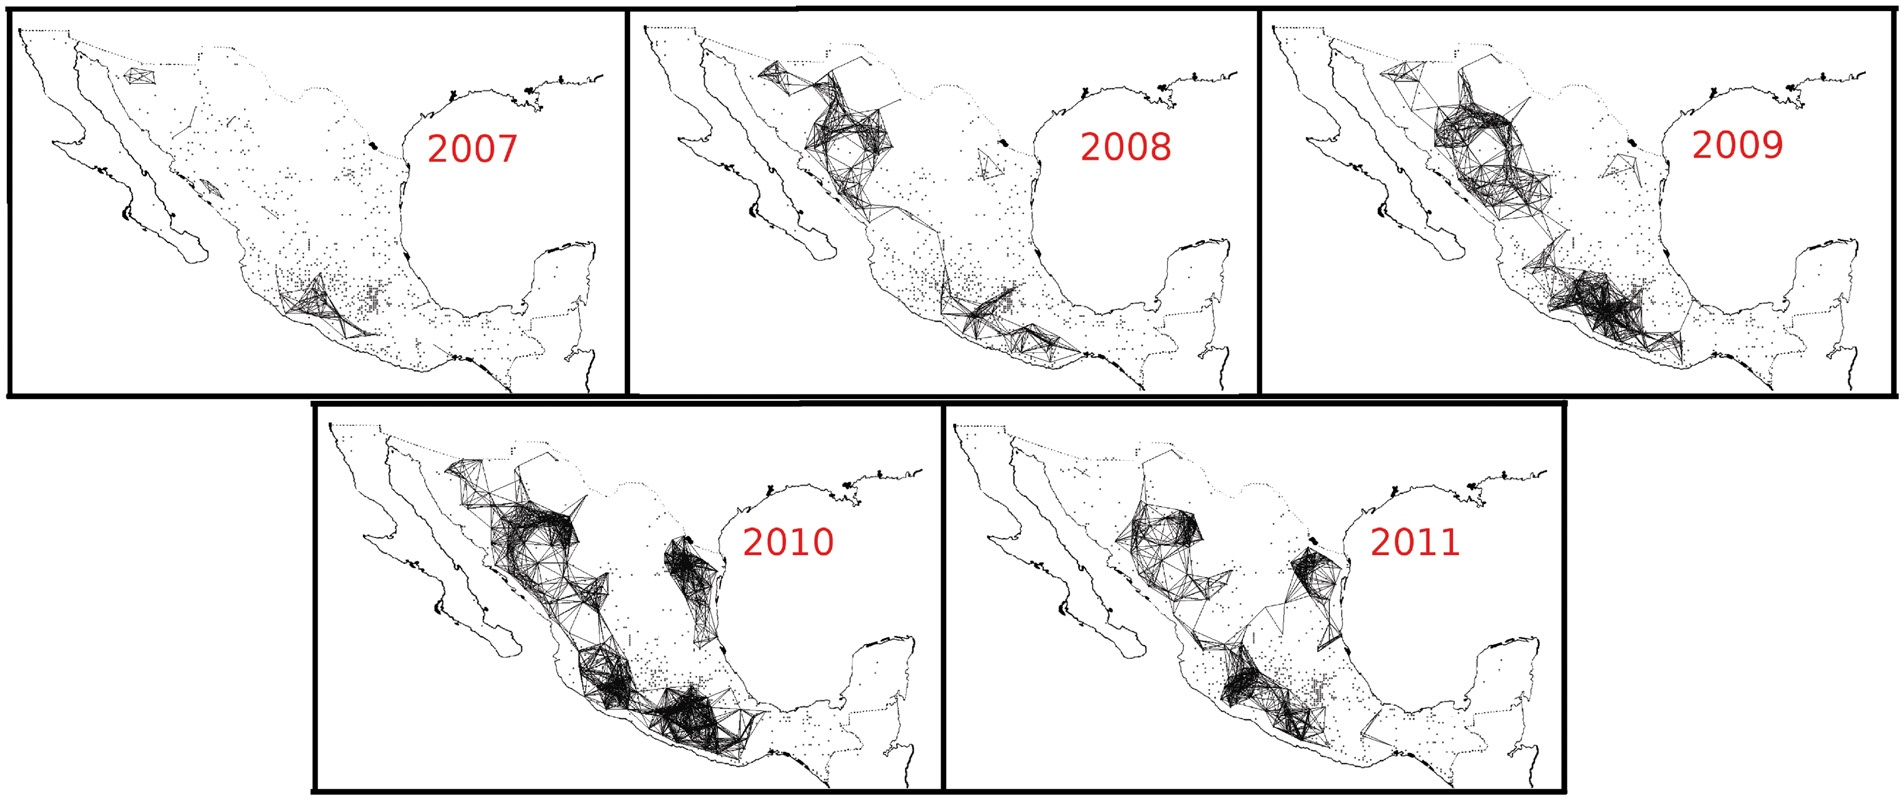
\includegraphics[scale=.72]{Figures/map1}
				\end{center}
				\tiny{Fuente: Espinal-Enr\'iquez J, Larralde H (2015)}
\end{frame}

\begin{frame}

\begin{center}
		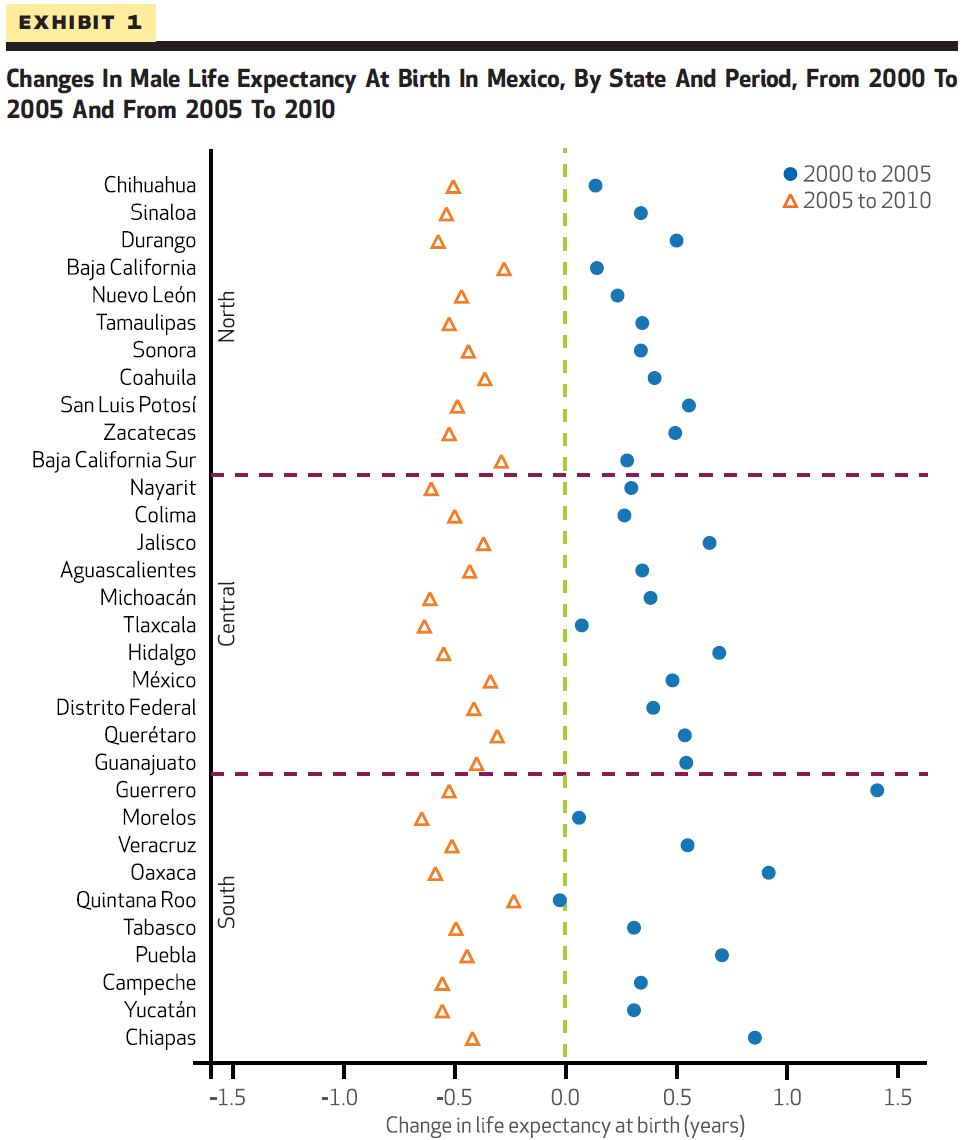
\includegraphics[scale=.24]{Figures/Fig3}
				\end{center}			
								\tiny{Fuente: Aburto, Beltr\'an-S\'anchez et al (2016)}
		

\end{frame}





\begin{frame}
\begin{center}
		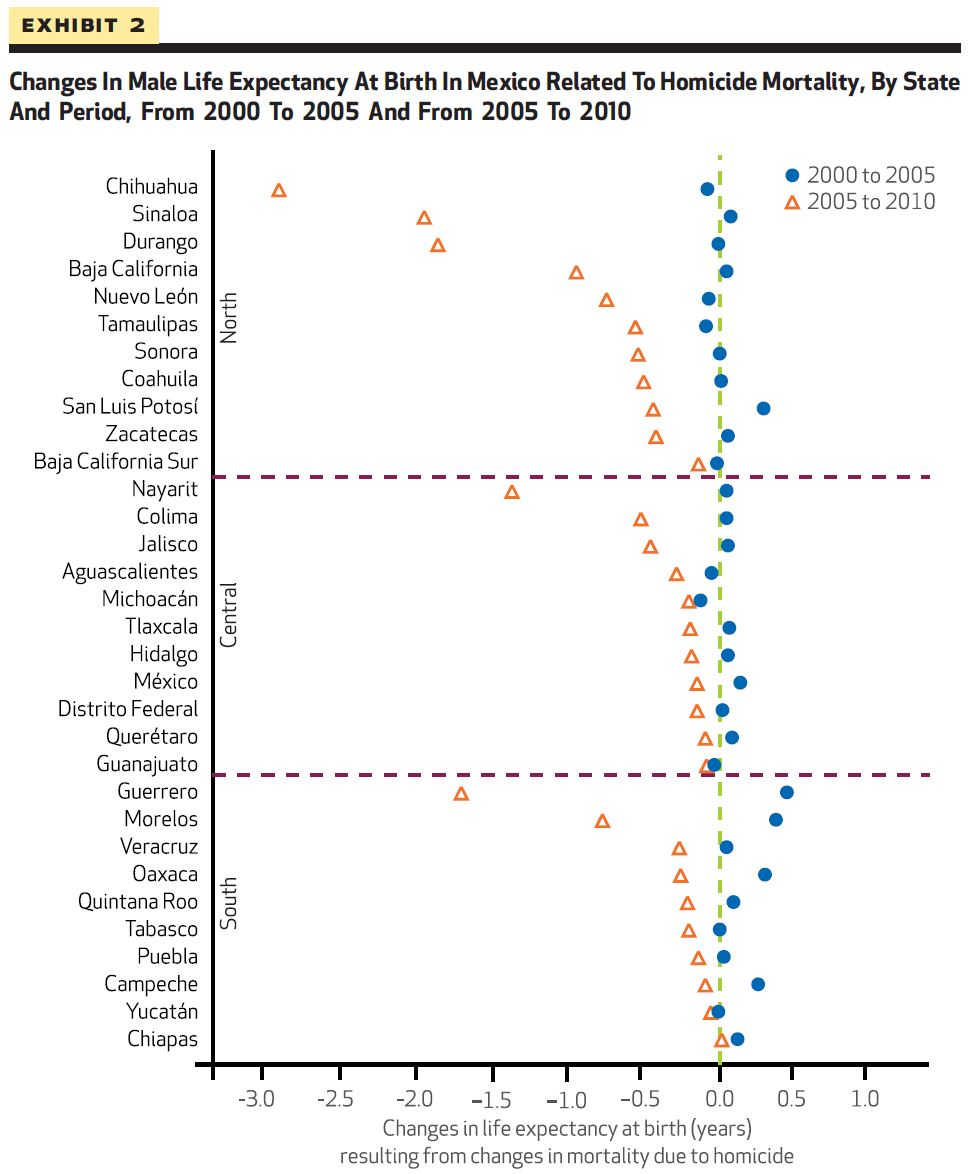
\includegraphics[scale=.24]{Figures/Fig4}
				\end{center}			
								\tiny{Fuente: Aburto, Beltr\'an-S\'anchez et al (2016)}
		

\end{frame}


\begin{frame}

\Large{
Tasas tres veces m\'as que las tropas de EU en Irak entre 2003 y 2006!
				\begin{center}
		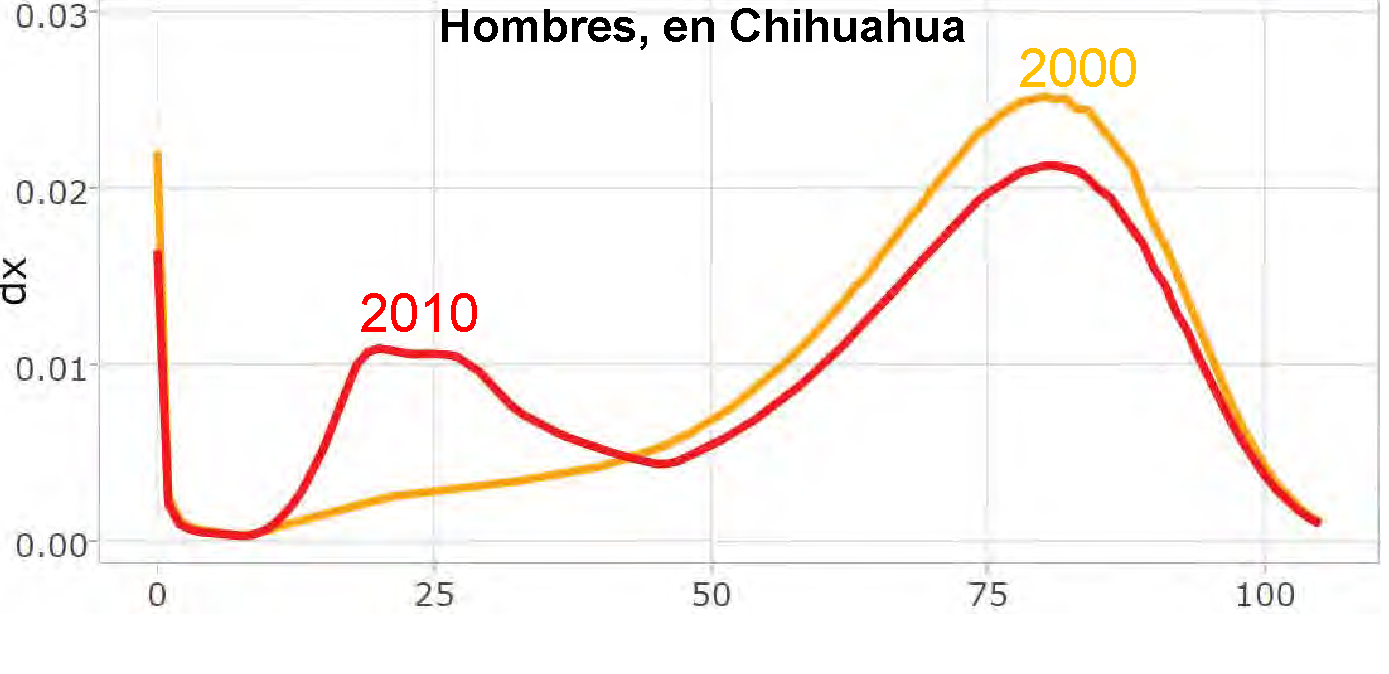
\includegraphics[scale=.45]{Figures/Distr_chihuahua}
				\end{center}				

}
\end{frame}


\begin{frame}
\Large{
		\begin{itemize}
		
		\item<1-> El efecto de la \textbf{violencia} va mucho m\'as all\'a que homicidios.
		
		\begin{itemize}
		\pause
		\large{
		\item Bajo rendimiento cognitivo de ni\~nos
		\item Incremento de ansiedad y depresi\'on
		\item Enfermedades del coraz\'on
		\item Migraci\'on
		\item Fecundidad
		\item Miedo y vulnerabilidad de la poblaci\'on				
		}
		\end{itemize}
		
		
		\end{itemize}
		
}

\end{frame}


\begin{frame}
\begin{center}
		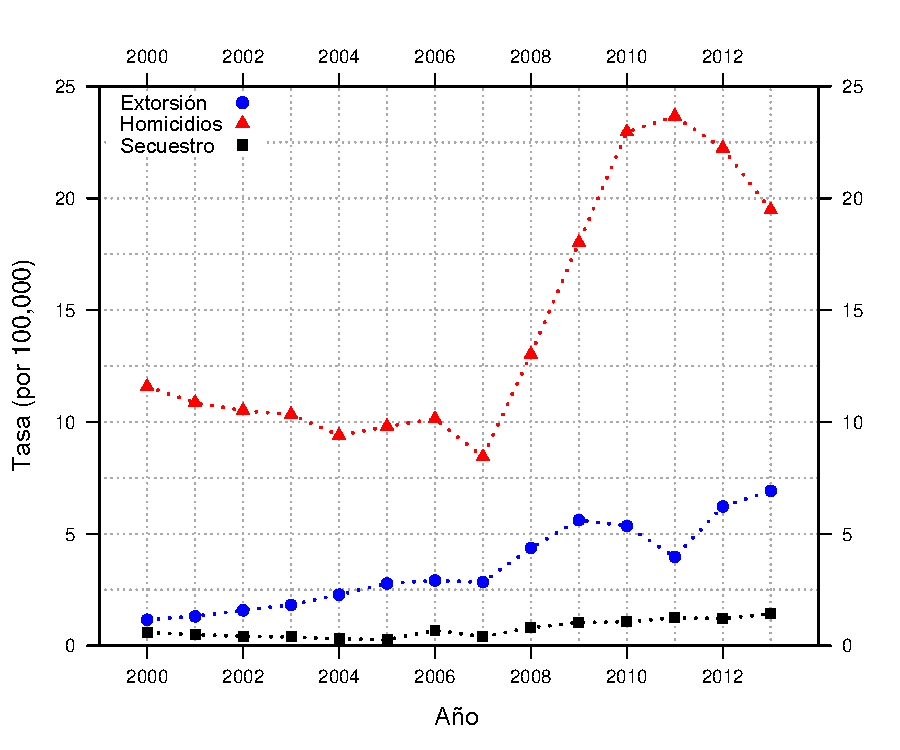
\includegraphics[scale=.52]{Figures/Fig5}
				\end{center}			
								\tiny{Fuente: Canudas-Romo, Aburto et al (2017)}
		

\end{frame}

\begin{frame}
\begin{center}
A\~nos persona vividos con vulnerabilidad/miedo a nivel estatal y hogar en 2005 y 2014.
		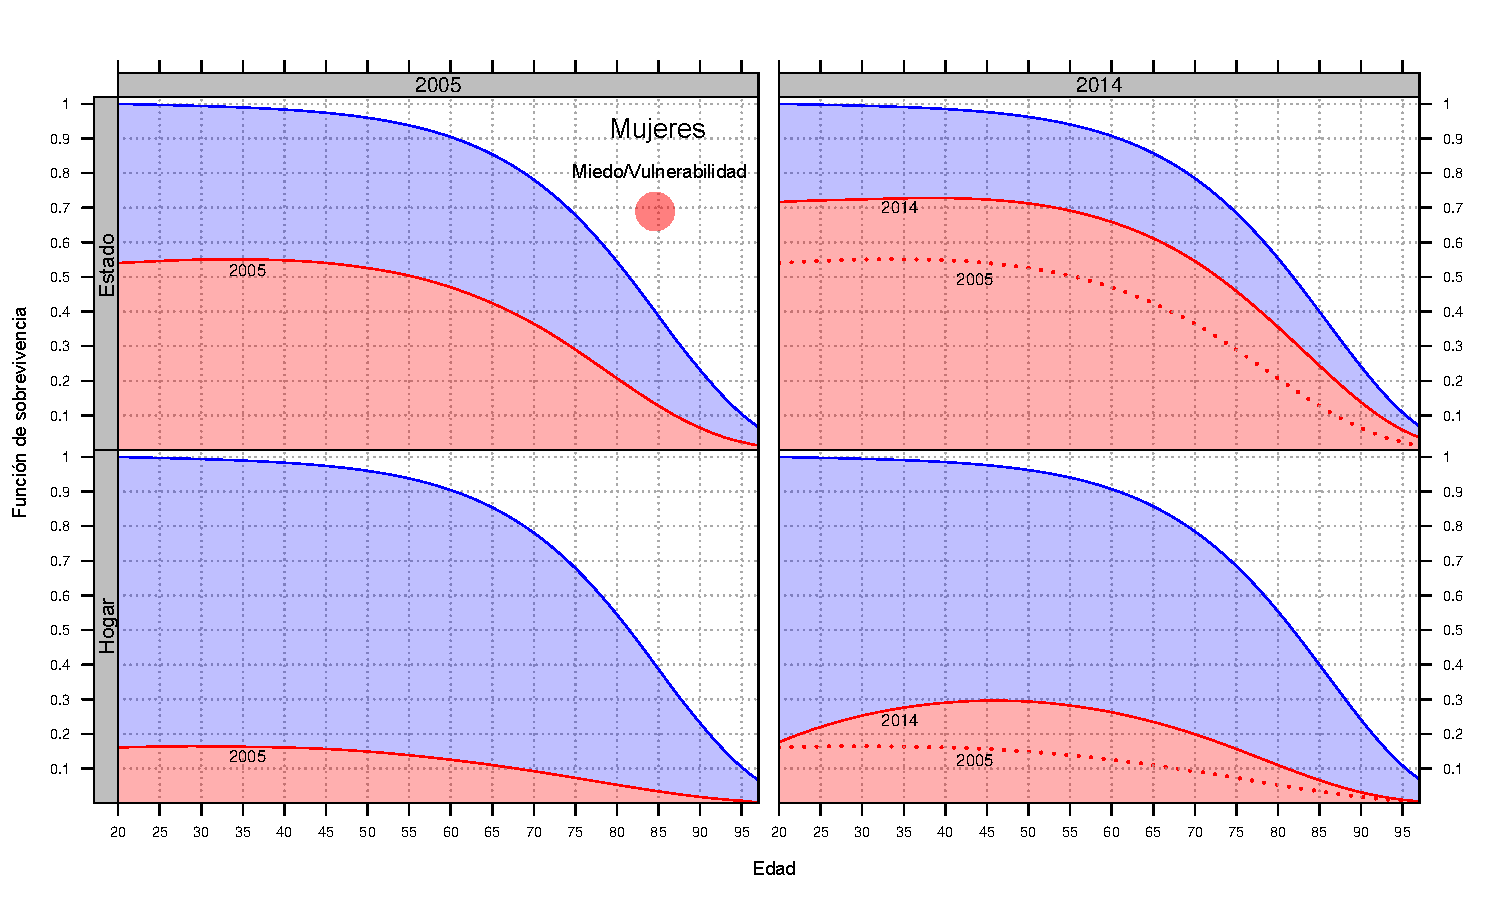
\includegraphics[scale=.45]{Figures/Fig6}
				\end{center}			
								\tiny{Fuente: Canudas-Romo, Aburto et al (2017)}
		

\end{frame}

\begin{frame}\frametitle{Mujeres}
\Large{
		\begin{itemize}
		
		\item<1-> $e_{20}$ en 2005 $\longrightarrow$ ~60
		\pause
        \item<1-> 51\% en vulnerabilidad/miedo a nivel estatal, 14\% en hogar
        \pause
        \item<1-> $e_{20}$ en 2014 $\longrightarrow$ ~60
		\pause
        \item<1-> 71\% en vulnerabilidad/miedo a nivel estatal, 26\% en hogar
		\end{itemize}
		\pause
\centering{		Perspectiva: 30.5 millones a\~nos-persona m\'as que en 2005}
		
		
}

\end{frame}


\begin{frame}\frametitle{Incertidumbre/desigualdad de la mortalidad}
\Large{
\begin{center}
		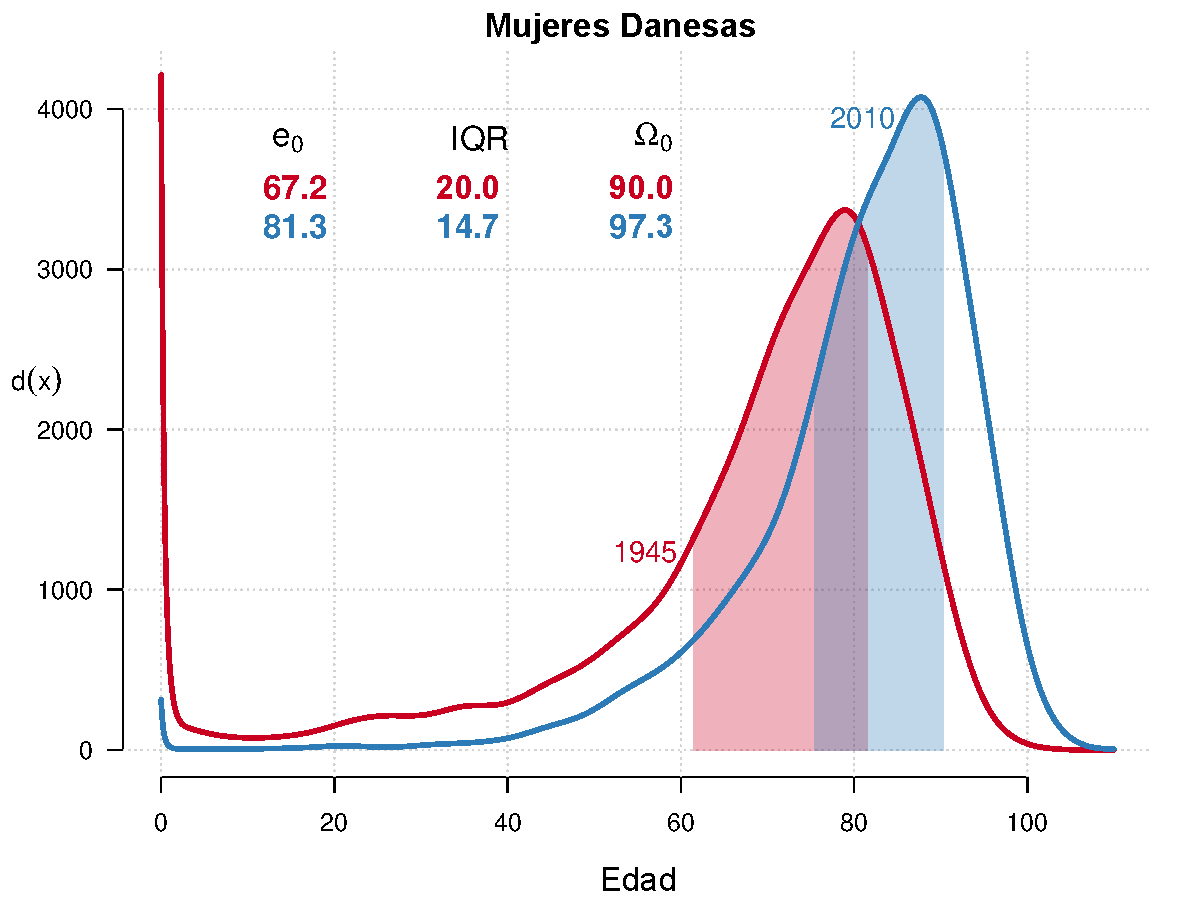
\includegraphics[scale=.45]{Figures/Fig0}
				\end{center}
}
\end{frame}


\begin{frame}\frametitle{Incertidumbre/desigualdad de la mortalidad}
\large{
		\begin{itemize}
		
		\item Medida de \textbf{incertidumbre} a nivel individual.
		\pause
     	\item Expresa una \textbf{desigualdad fundamental} a nivel de poblaci\'on.
\pause
		\item Tomamos decisiones bas\'andonos en \textbf{ambos}.		
		\pause				
		\end{itemize}
}
\Large{
\begin{center}
Cu\'al es el efecto de homicidios en adultos j\'ovenes?.
\end{center}
}
\end{frame}




\begin{frame}\frametitle{C\'omo medirlo?}
\Large{
$e^{\dagger}\longrightarrow  $ promedio de vida perdida al morir.

\begin{itemize}
\item F\'acil de interpretar (a\~nos).
\item Relacionado con disparidad/entrop\'ia.
\item Cuantificar el efecto de distintas edades y homicidios.

\end{itemize}

}
\end{frame}




\begin{frame}





\Large{
Se acuerdan del estancamiento 2000-10?

				\begin{center}
		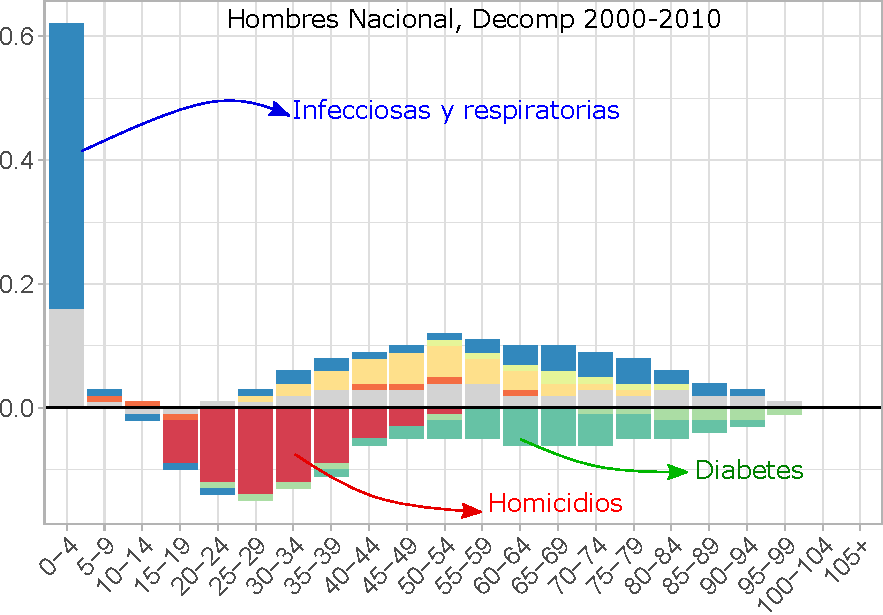
\includegraphics[scale=.65]{Figures/Fig_1}
				\end{center}
				

}
\end{frame}


\begin{frame}

\Large{
Now $e^\dagger \backsim$ 15y

				\begin{center}
		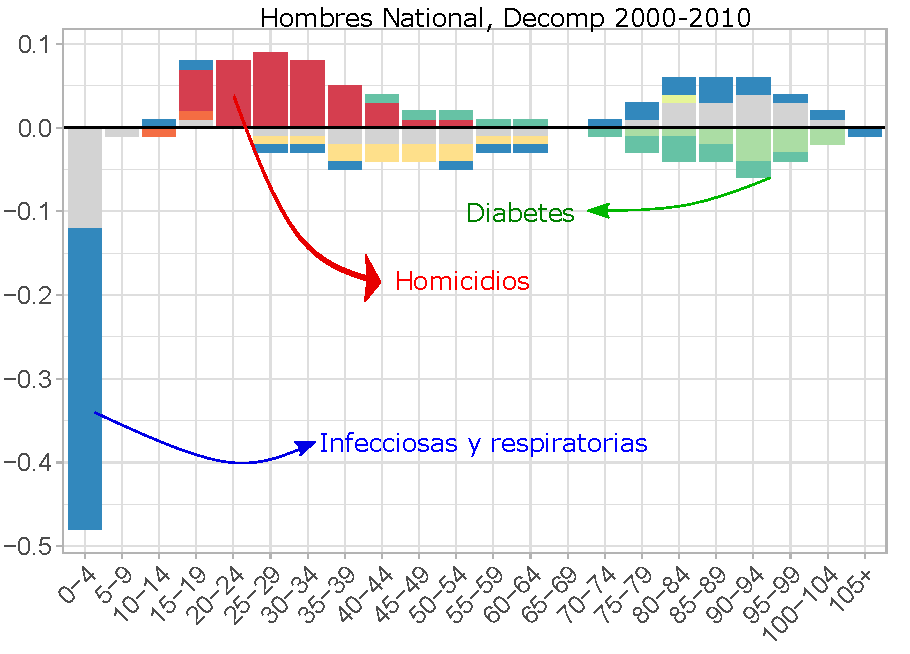
\includegraphics[scale=.65]{Figures/Cause_ed_decomp_Males}
				\end{center}				

}
\end{frame}


\begin{frame}\frametitle{1995-2015}

\Large{
				\begin{center}
		\hbox{\hspace{-2em}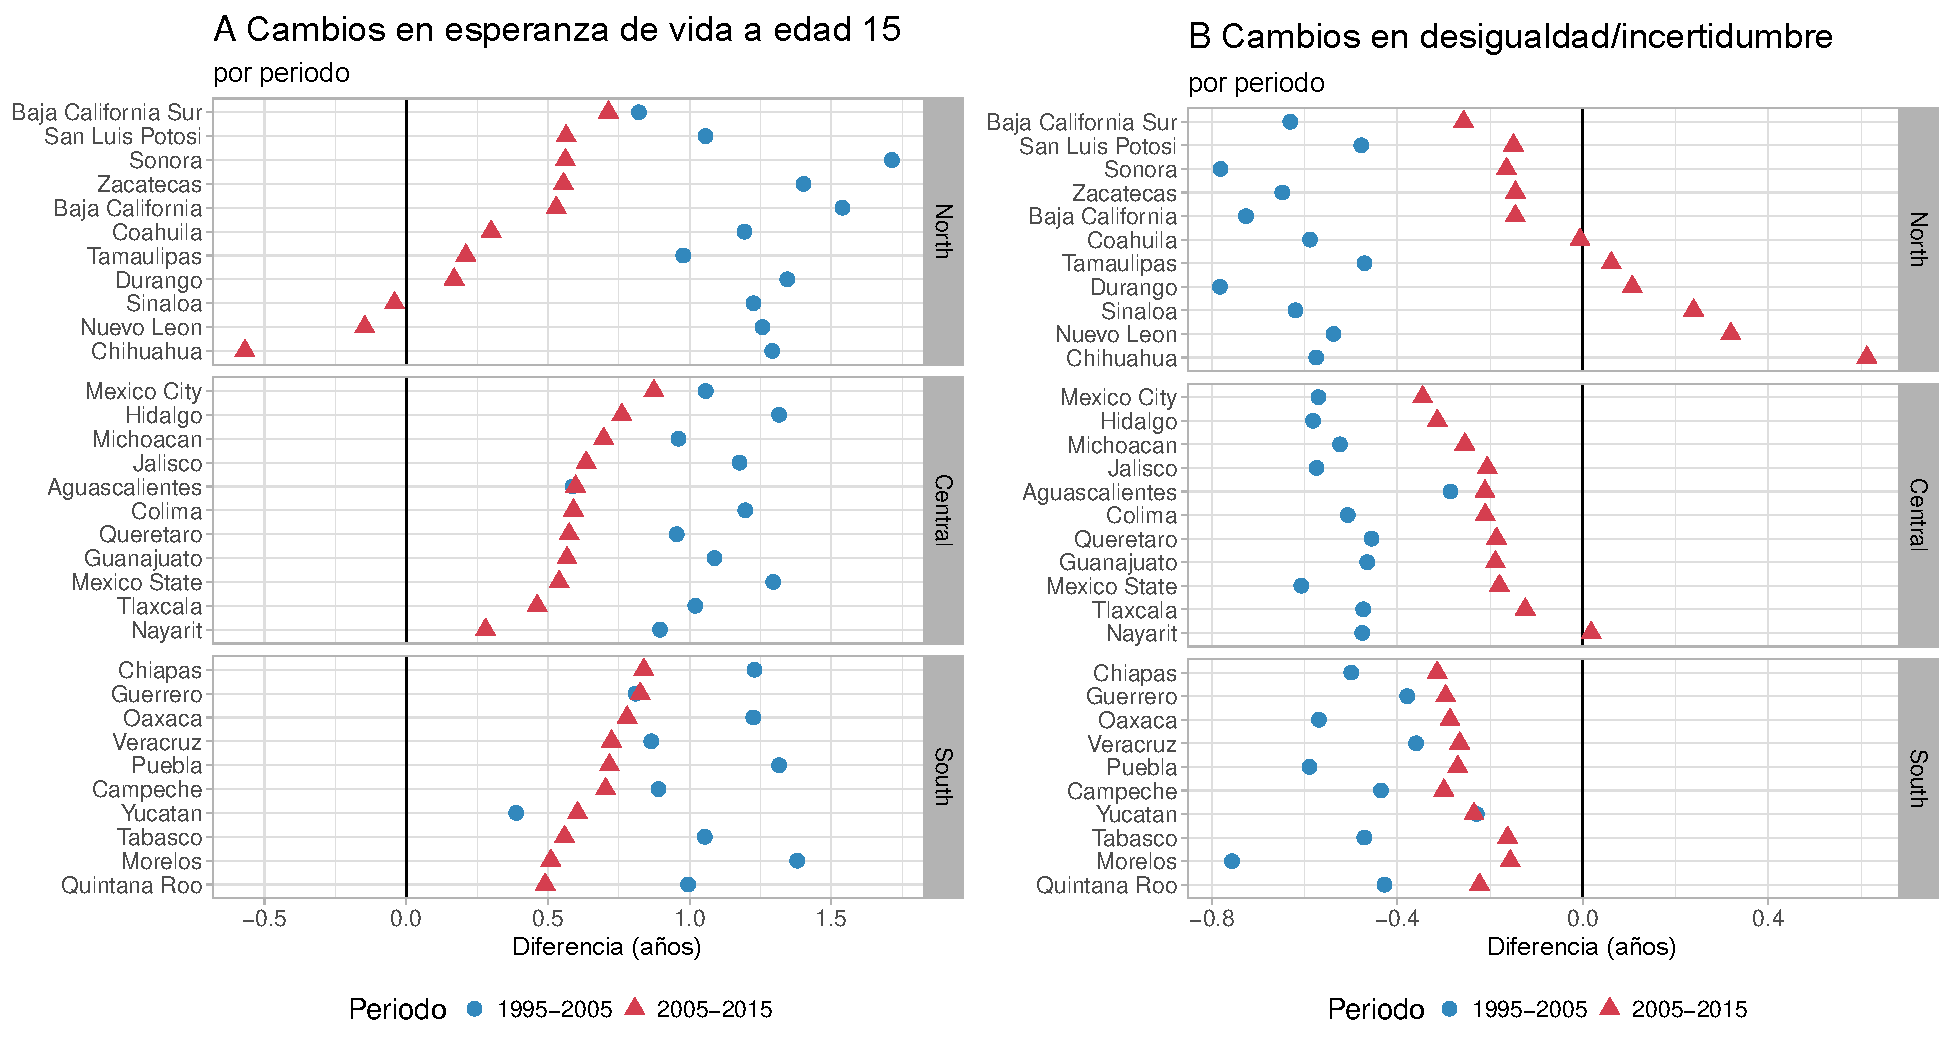
\includegraphics[scale=.38]{Figures/Changes_2005-15}}
				\end{center}		
\vspace{-2em}\tiny{Fuente: Aburto, Beltr\'an-S\'anchez (forthcoming)}		

}
\end{frame}

\begin{frame}
\Large{
				\begin{center}
		\hbox{\hspace{-2em}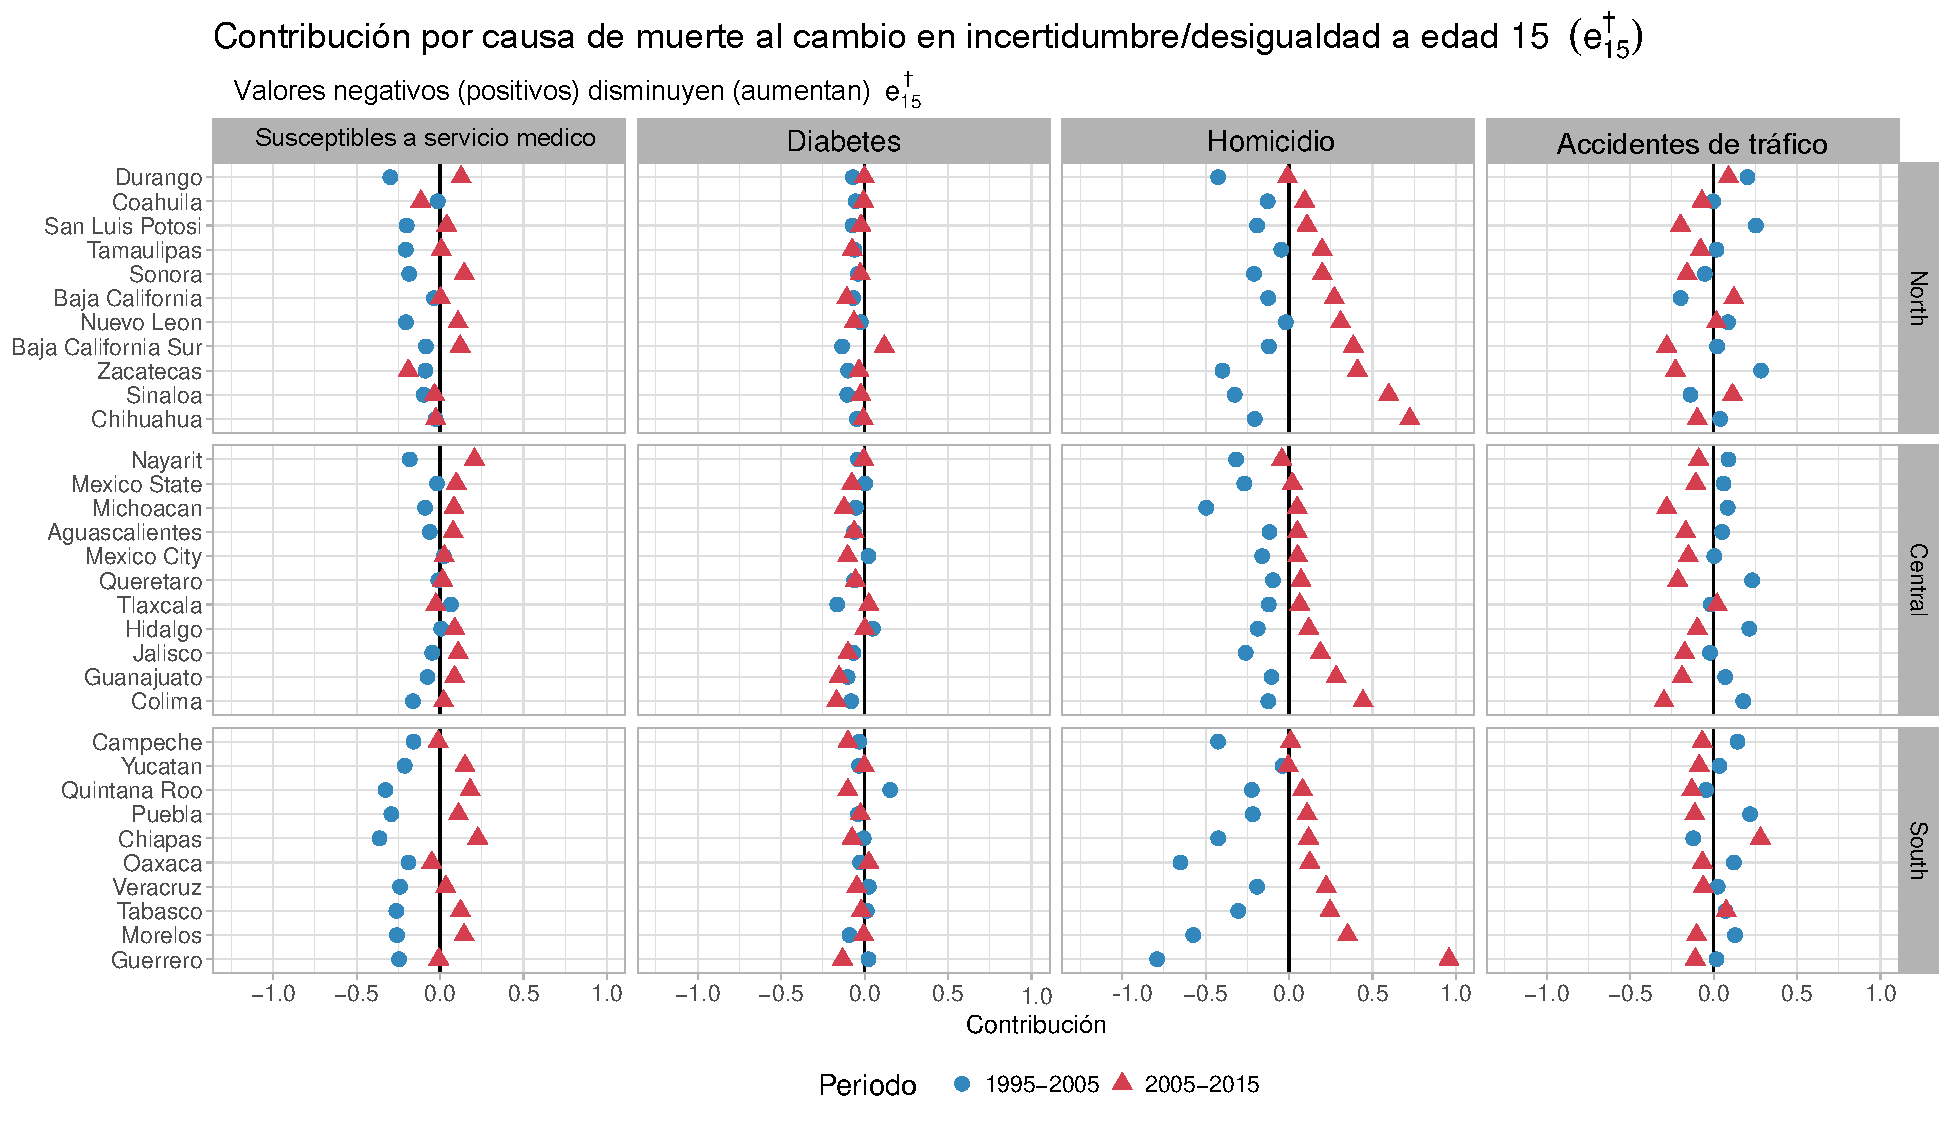
\includegraphics[scale=.38]{Figures/Changes_2005-15b}}
				\end{center}				
\vspace{-2em}\tiny{Fuente: Aburto, Beltr\'an-S\'anchez (forthcoming)}		

}
\end{frame}

\begin{frame}
\Large{

\begin{center}		
\animategraphics[autoplay, scale=0.4]{3}{Figures/Cause_ed_decomp_Males_states}{1}{33}
				\end{center}
				
}
\end{frame}


\begin{frame}
\Large{
				\begin{center}
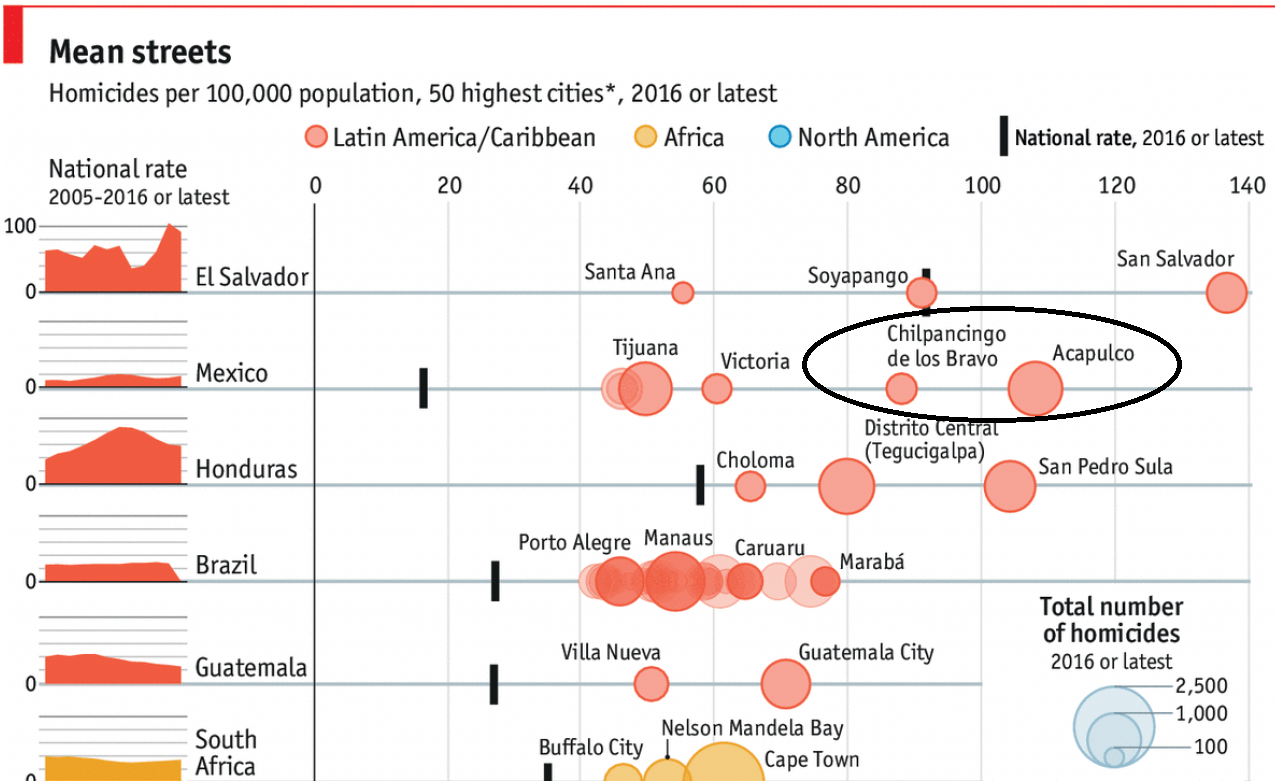
\includegraphics[scale=.4]{Figures/Capture}
				\end{center}				
}
\end{frame}

\section{Contexto Am\'erica Latina}

\begin{frame}
\Huge{
\begin{center}
{\fontsize{70}{80}\selectfont $\backsim$ 2,000,000}\\
15-30

\end{center}
}
\end{frame}

\begin{frame}
\Huge{
\begin{center}
{\fontsize{70}{80}\selectfont 77\%}\\
Hombres

\end{center}
}
\end{frame}


\begin{frame}
\Huge{
\begin{center}
{\fontsize{70}{80}\selectfont 35\% Homicidios}\\
(+ de medio mill\'on)

\end{center}
}
\end{frame}


\begin{frame}
\Large{
				\begin{center}
				Esperanza de vida en Am\'erica Latina
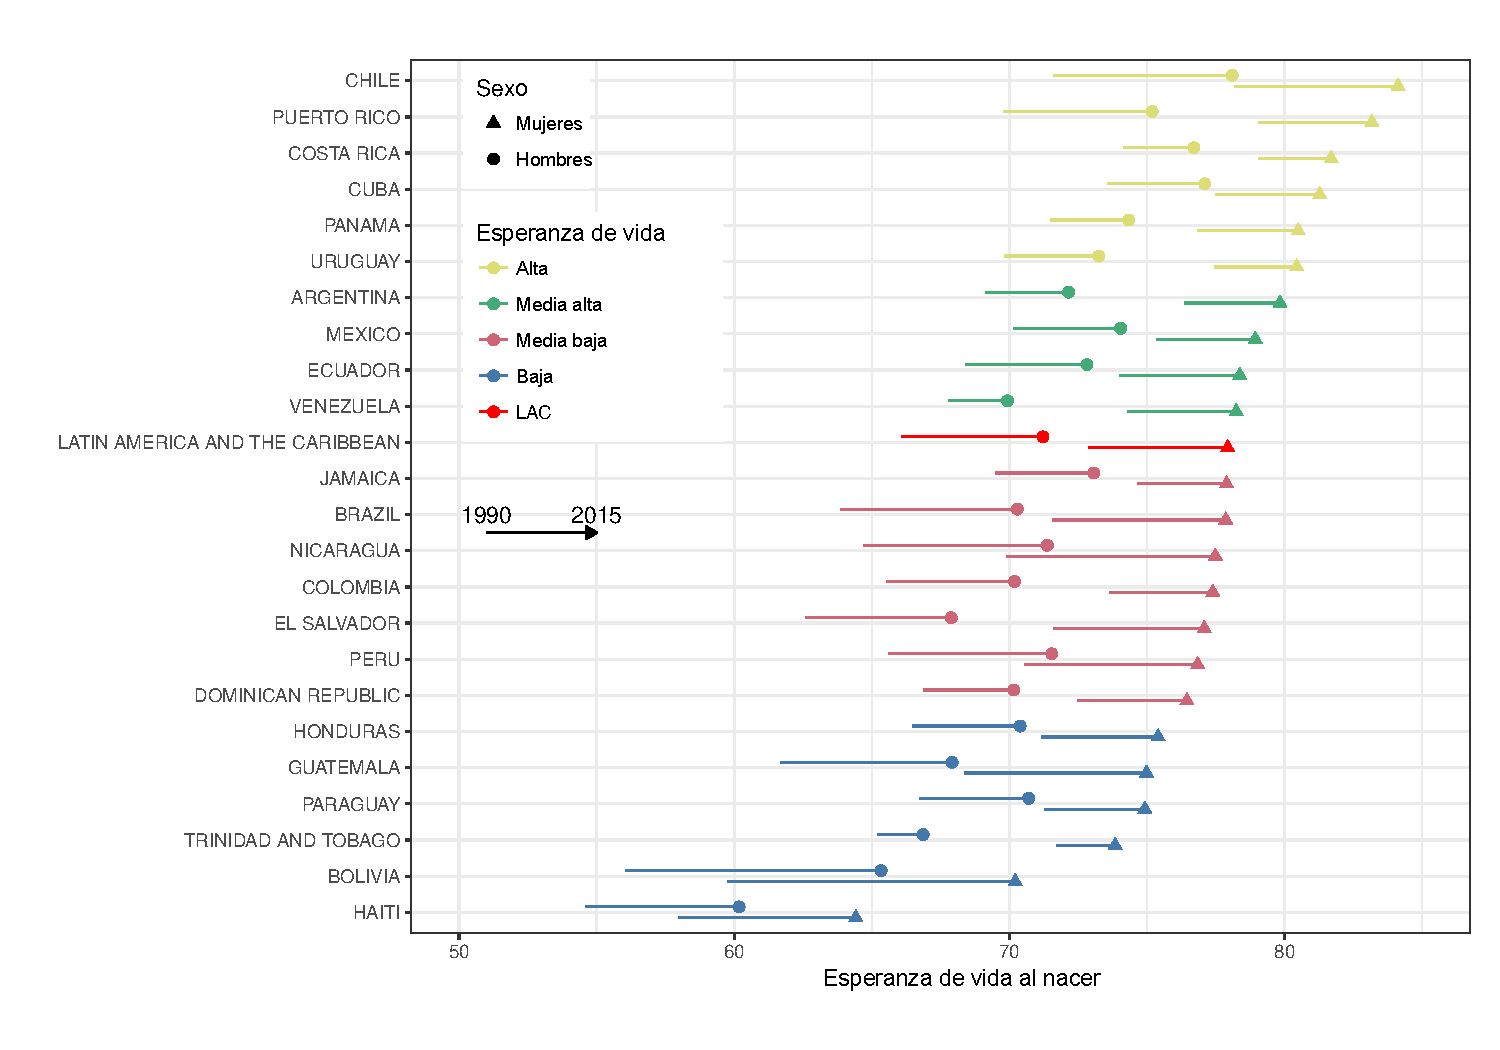
\includegraphics[scale=.4]{Figures/Fig1_V4}
				\end{center}				
}
\vspace{-2em}\tiny{Fuente: Canudas-Romo, Aburto (2018)}		
\end{frame}


\begin{frame}
Venezuela
\Large{
				\begin{center}
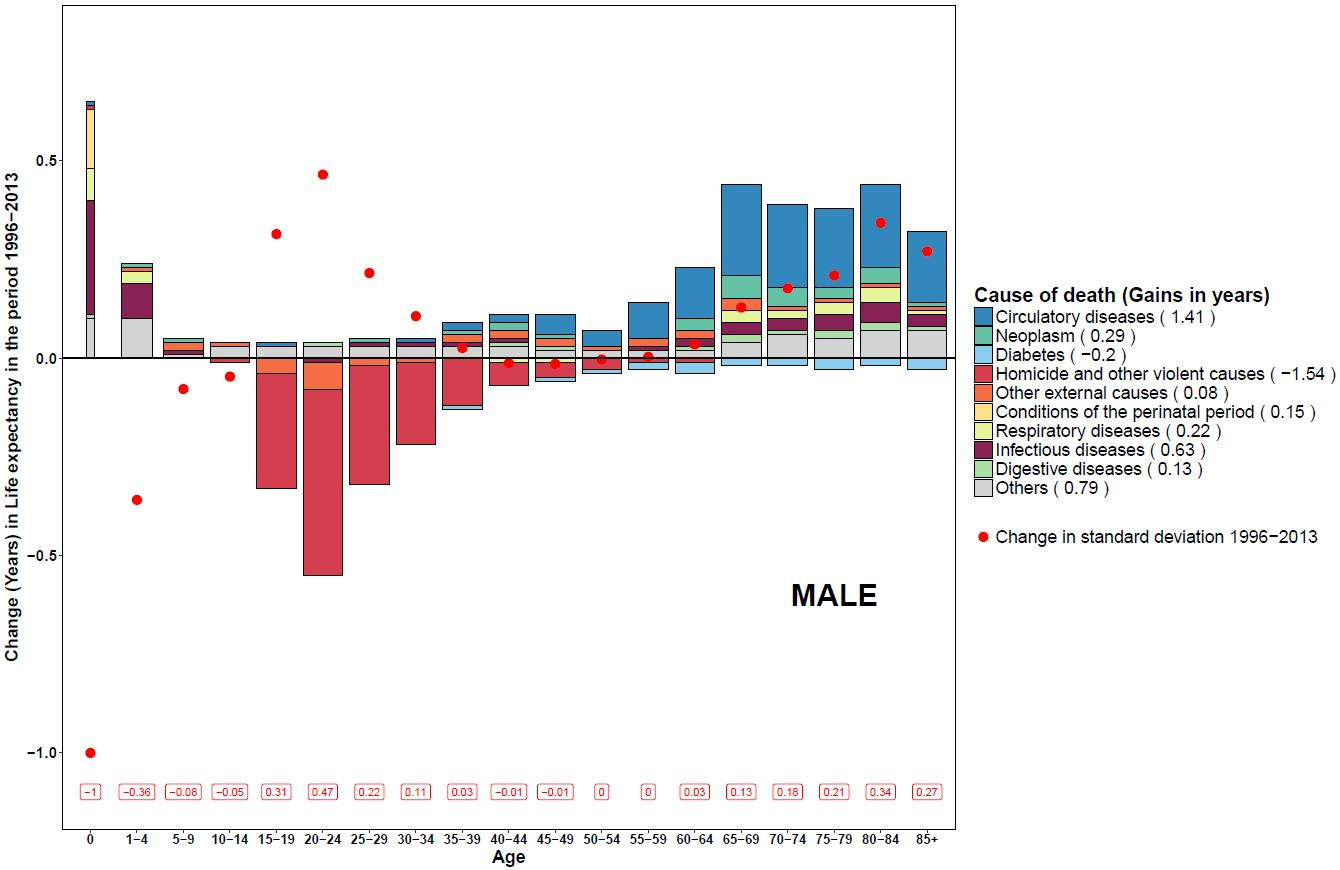
\includegraphics[scale=.37]{Figures/Venezuela}
				\end{center}				
}
\vspace{-1em}\tiny{Fuente: Garc\'ia, Aburto (Preliminar)}		
\end{frame}



\begin{frame}
\Large{
				\begin{center}
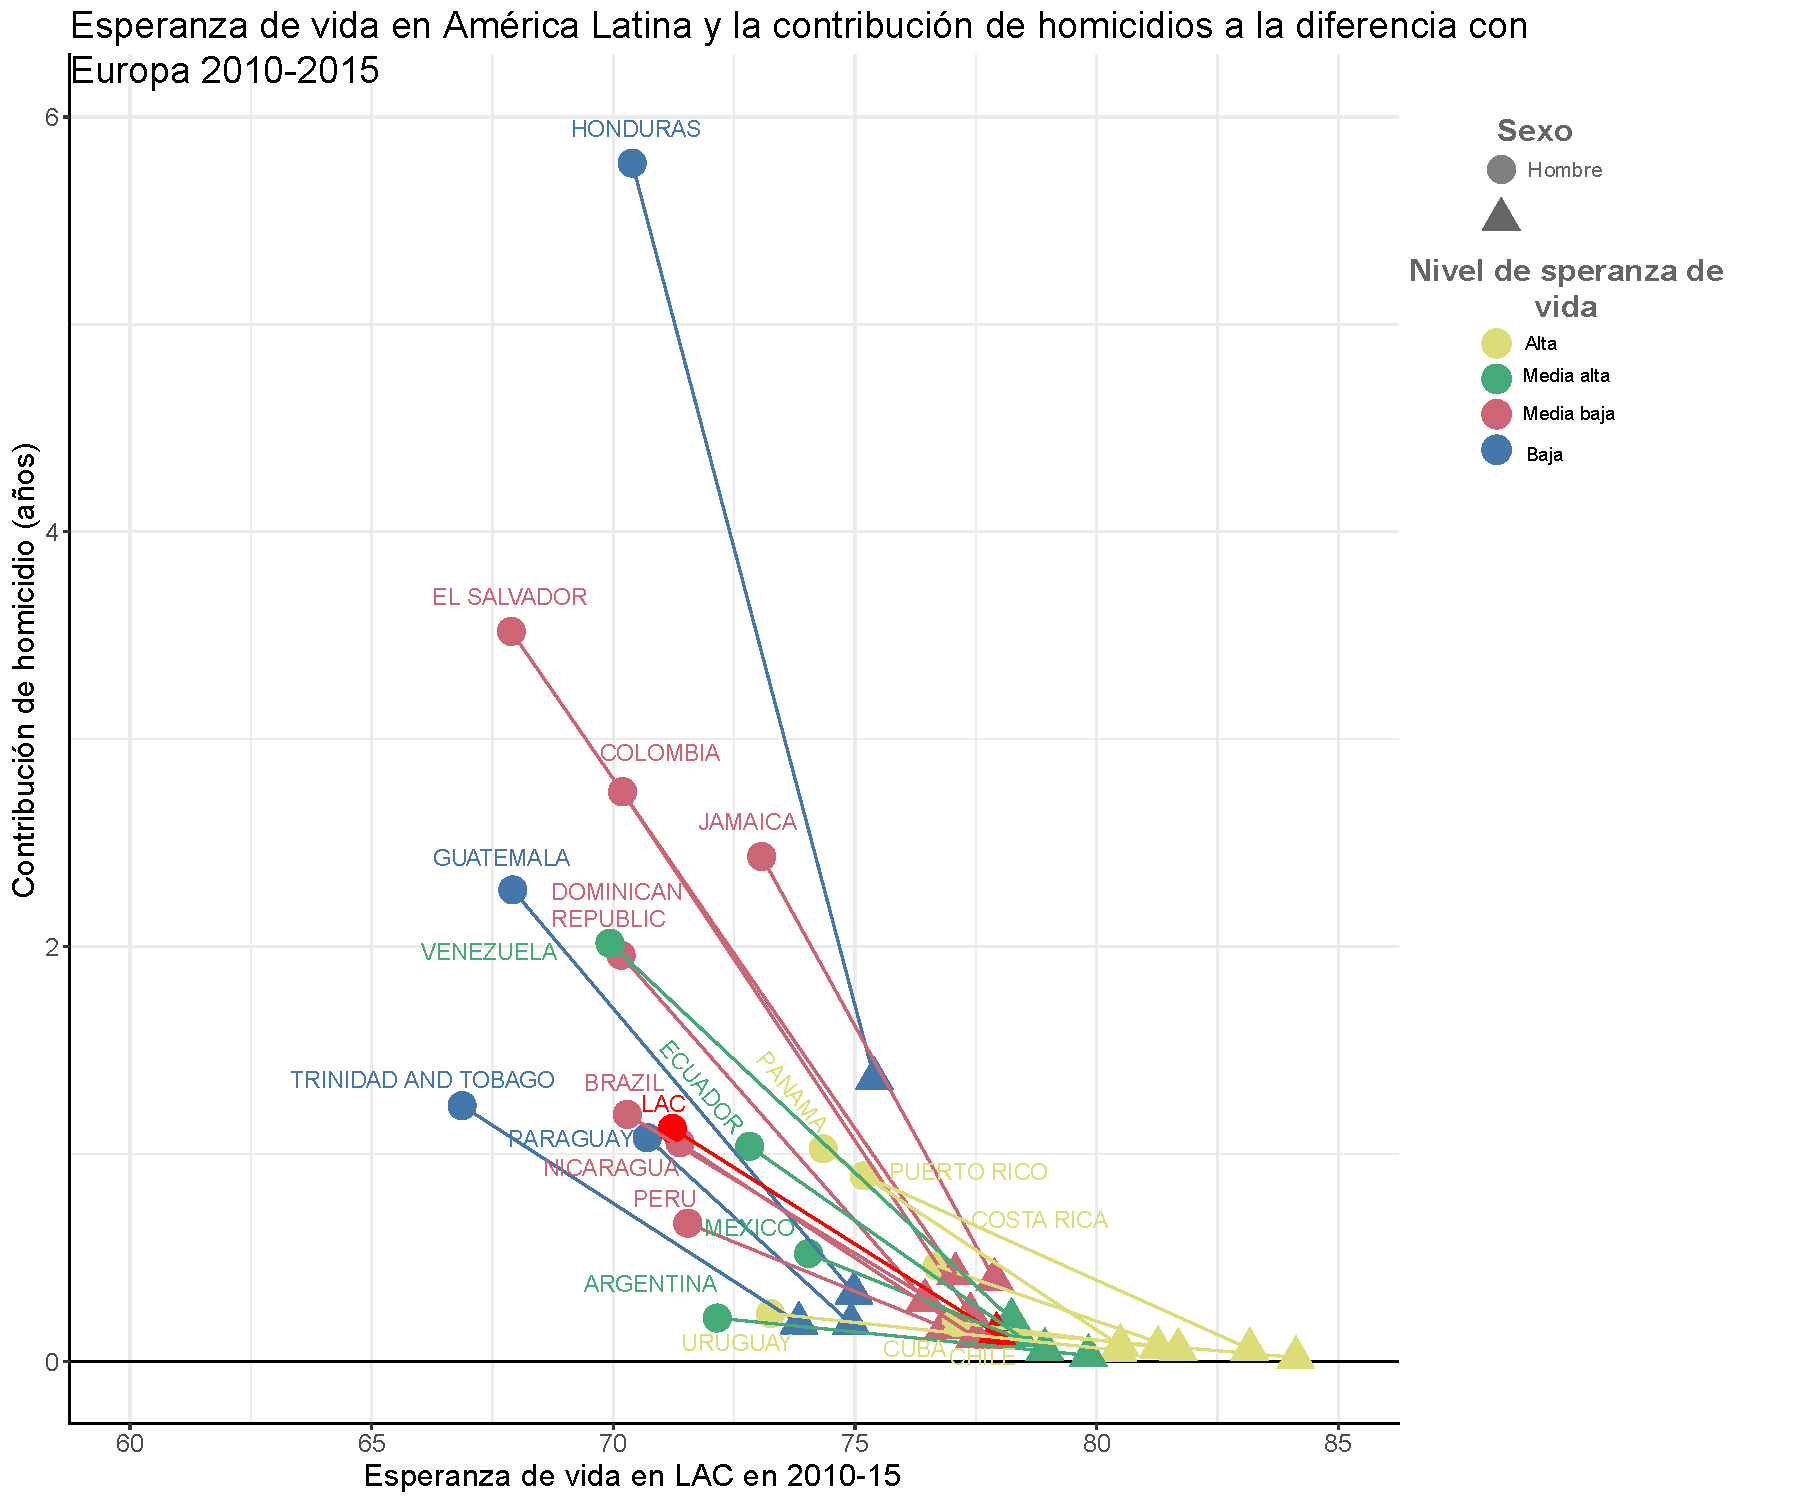
\includegraphics[scale=.31]{Figures/Fig2_V4}
				\end{center}				
}
\end{frame}



%%%%%%%%%%%%%%%%%%%%%%%%%%%%%%%%%%%%%%%%%%%%%%%%%%%%%%%%%%%%%%%%%%%%%%%%

%%%%%%%%%%%%%%%%%%%%%%%%%%%%%%%%%%%%%%%%%%%%%%%%%%%%%%%%%%%%%%%%%%%%%%%%
\section{Conclusi\'on}
\begin{frame}
 \begin{center}
	\begin{center}
	\huge{ \textbf{Retos de M\'exico: Violencia y Desigualdad}}
	\end{center}
	
	\bigskip
	\bigskip
M\'as informaci\'on:

jmaburto@health.sdu.dk 

\faTwitter \quad  @jm\_aburto 

\faGithub \quad @jmaburto 

Shinnyapp: \url{https://jmaburto.shinyapps.io/LVMx_App/}\\
\url{https://wb-lac.shinyapps.io/lac_diversity/}


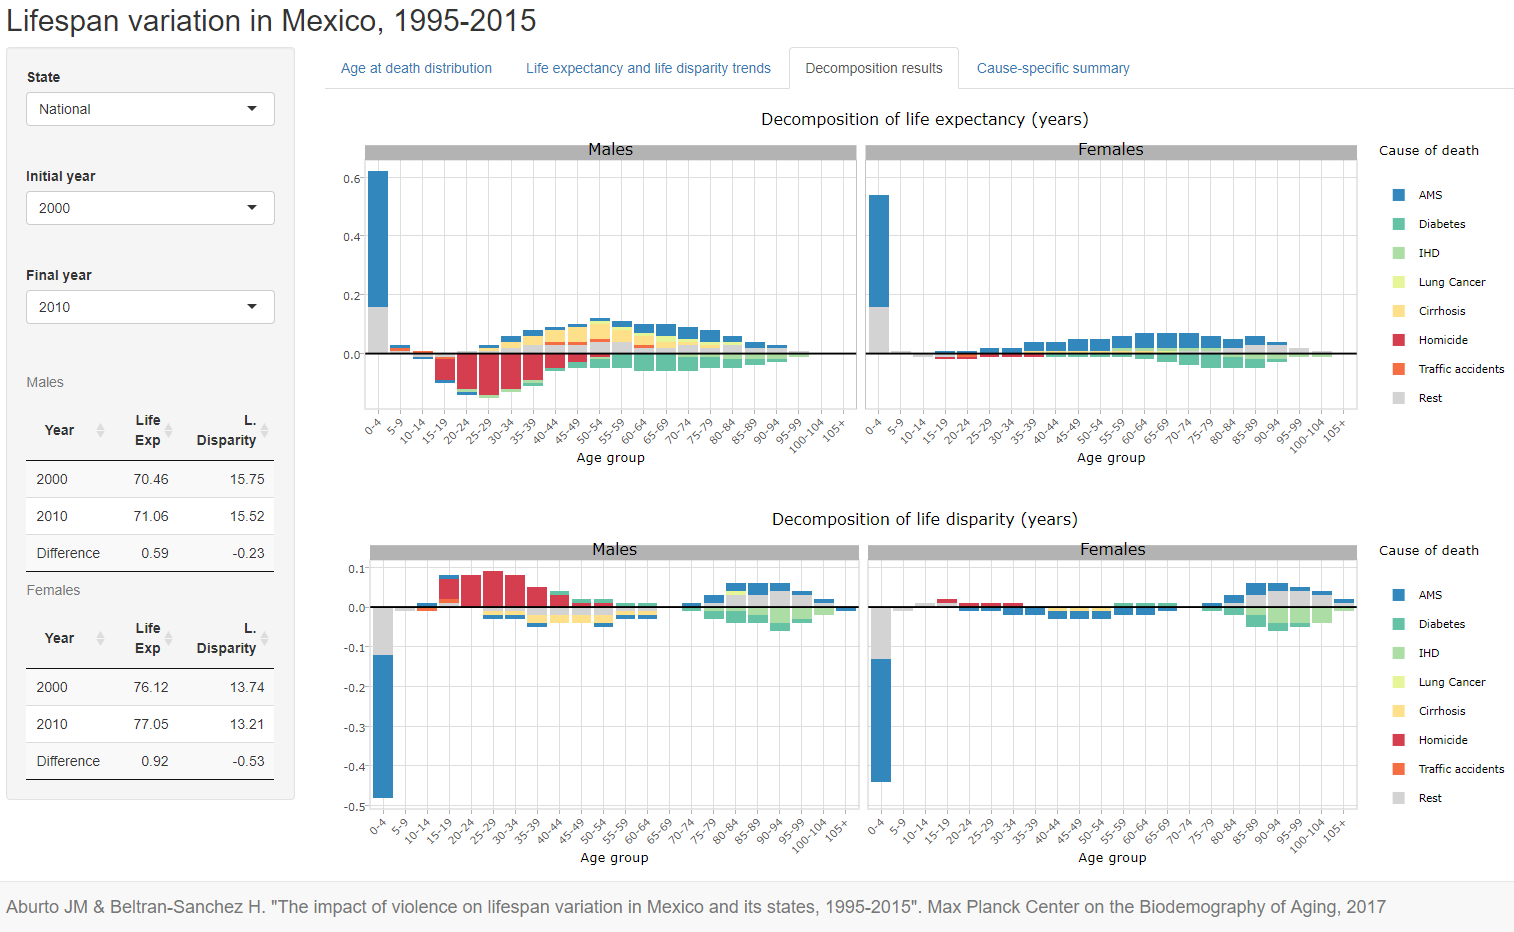
\includegraphics[scale=0.1]{Figures/Shinnyapp_fig} \\   

 

\end{center}
 
 

\end{frame}



\end{document}
	

